\newpage
\section{Storage, Networks and Other Peripherals}

\subsection{Introduction}
Performance of I/O system depends on:
\begin{itemize}\small
    \item Connection between devices and the system
    \item The memory hierarchy
    \item The operating system
\end{itemize}


\subsubsection{Typical I/O Devices}
\begin{figure}[!htb]
    \centering
    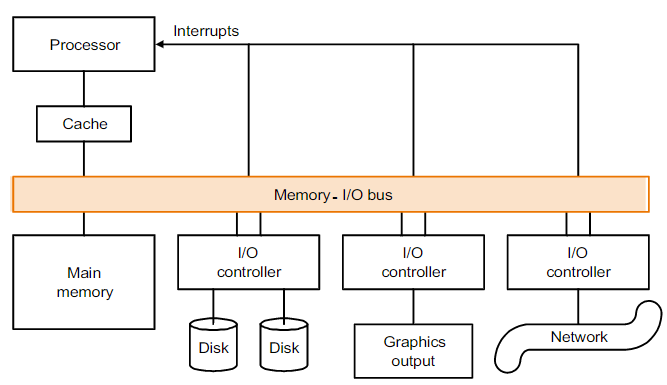
\includegraphics[width=0.42\textwidth]{CO6/Typical IO Devices}
    \caption{Typical IO Devices}
\end{figure}

\subsubsection{Three Characters of I/O}
\begin{enumerate}
    \item Behavior: Input (read once), output (write only, cannot read), or storage (can be reread and usually rewritten)
    \item Partner: Either a human or a machine is at the other end of the I/O device, either feeding data to input or reading data from output.
    \item Data rate: The peak rate at which data are transferred between the I/O device and the main memory or processor.    
\end{enumerate}

\subsubsection{I/O Performance Depends on the Application}
\begin{itemize}
    \item Throughput
    \item Response time
    \item Both throughput and response time
\end{itemize}

\subsubsection{Amdahl's Law (阿姆达尔定律)}
Sequential part can limit speedup. Remind us that ignoring I/O is dangerous. 

\subsection{Disk Storage and Dependability}
\begin{itemize}\small
    \item  Magnetic disks: Hard disks
    \subitem (physically) larger
    \subitem higher storage volume
    \subitem reliable storage
    \subitem more than one platter
    \item SSD = Solid State Drive
    \subitem No mechanical part (all implemented in chip)
    \subitem $> 100X$ faster
\end{itemize}

\subsubsection{The Organization of Hard Disk}
\begin{itemize}\small
    \item platters: disk consists of a collection of platters, each of which has two recordable disk surfaces
    \item tracks: each disk surface is divided into concentric circles
    \item sectors: each track is in turn divided into sectors, which is the smallest unit that can be read or written
\end{itemize}

\begin{figure}[!htb]
    \centering
    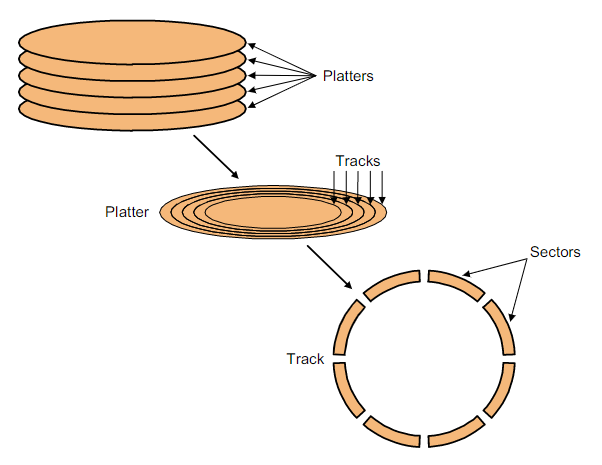
\includegraphics[width=0.309\textwidth]{CO6/The Organization of Hard Disk}
    \caption{The Organization of Hard Disk}
\end{figure}

\subsubsection{To Access Data on Disk}
\begin{itemize}\small
    \item Seek: position read/write head over the proper track
    \item Rotational latency: wait for desired sector
    \item Transfer time: time to transfer a sector (1 KB/sector) of data
    \item Disk controller: control the transfer between the disk and the memory
\end{itemize}

\subsubsection{Flash Storage}
Nonvolatile solid-state storage.

Flash Types:
\begin{itemize}\small
    \item NOR flash: bit cell like a NOR gate
    \item NAND flash: bit cell like a NAND gate
\end{itemize}

\subsubsection{Dependability, Reliability, Availability}
Computer system dependability is the quality of delivered service such that reliance can justifiably be placed on this service.

\paragraph{Measure}
\begin{itemize}
    \item MTTF (Mean Time to Failure)
    \item MTTR (Mean Time to Repair)
    \item MTBF (Mean Time Between Failures)
    \subitem = MTTF+ MTTR
    \item Availability
    \begin{align*}
        \text{Availability}=\frac{\text{MTTF}}{\text{MTTF}+\text{MTTR}}
    \end{align*}
\end{itemize}

\paragraph{Array Reliability}
\begin{figure}[!htb]
    \centering
    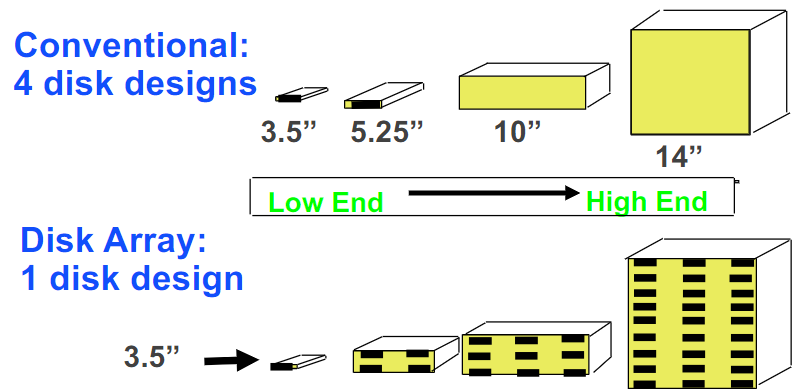
\includegraphics[width=0.42\textwidth]{CO6/Use Arrays of Small Disks}
    \caption{Use Arrays of Small Disks}
\end{figure}
\begin{itemize}
    \item Reliability of $N$ disks $=$ Reliability of 1 Disk$/$N
    \item AFR (annual failure rate) = percentage of devices to fail per year. 
\end{itemize}

Reliability can be measured by ``nines of availability'' per year
\begin{figure}[!htb]
    \centering
    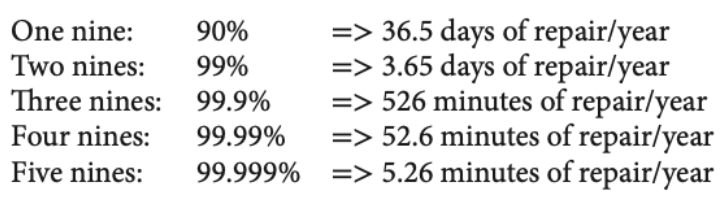
\includegraphics[width=0.309\textwidth]{CO6/Measure Reliability}
    \caption{Measure Reliability}
\end{figure}

\paragraph{Three Ways to Improve MTTF}
\begin{enumerate}\small
    \item Fault avoidance:
    preventing fault occurrence by construction
    \item Fault tolerance:
    using redundancy to allow the service to comply with the
    service specification despite faults occurring, which applies
    primarily to hardware faults
    \item Fault forecasting:
    predicting the presence and creation of faults, which applies
    to hardware and software faults
\end{enumerate}

\subsubsection{RAID: Redundant Arrays of (Inexpensive) Disks}
A disk arrays replace larger disk

\paragraph{RAID 0: No Redundancy}
Data is striped across a disk array but there is no redundancy to tolerate disk failure.

\paragraph{RAID 1: Disk Mirroring/Shadowing}
Each disk is fully duplicated onto its ``mirror''. 

\begin{figure}[!htb]
    \centering
    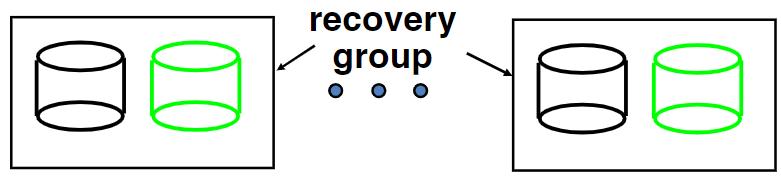
\includegraphics[width=0.309\textwidth]{CO6/RAID 1}
    \caption{RAID 1}
\end{figure}

\paragraph{RAID 3: Bit-Interleaved Parity Disk}

$P$ contains sum of other disks per stripe mod 2 (``parity'').  If disk fails, subtract $P$ from sum of other disks to find missing information. 

\begin{figure}[!htb]
    \centering
    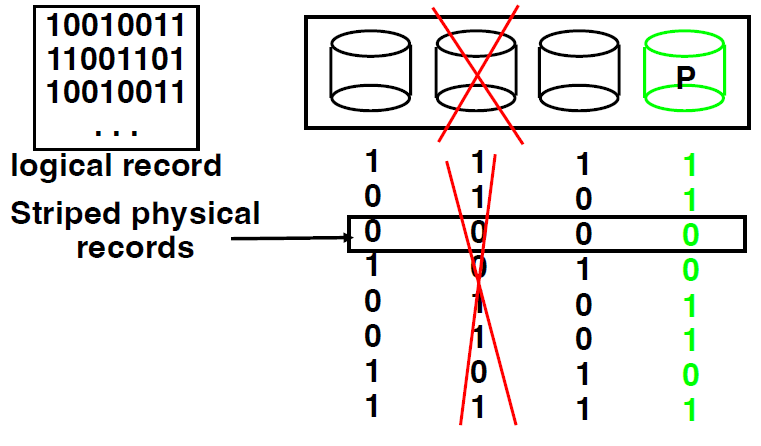
\includegraphics[width=0.309\textwidth]{CO6/RAID 3}
    \caption{RAID 3}
\end{figure}


\paragraph{RAID 4:Block-Interleaved Parity}
Every sector has an error detection field. Rely on error detection field to catch errors on read, not on the parity disk. 

\begin{figure}[!htb]
    \centering
    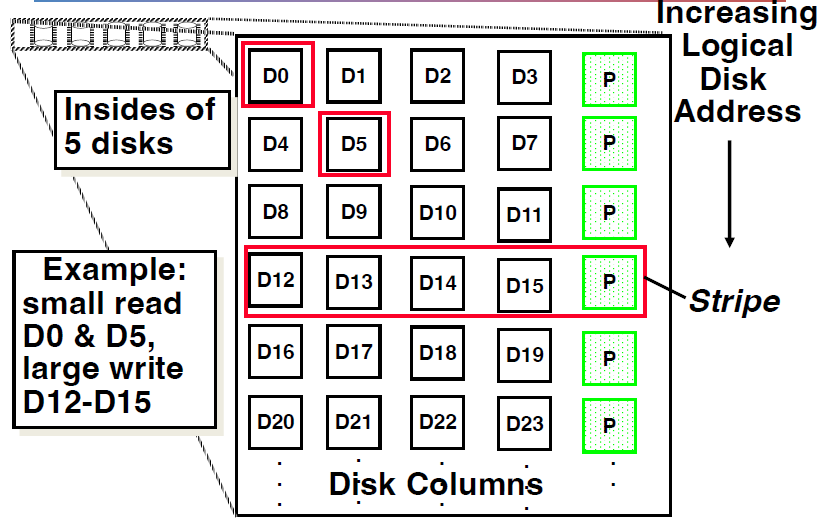
\includegraphics[width=0.309\textwidth]{CO6/RAID 4}
    \caption{RAID 4}
\end{figure}

Problems of Disk Arrays: Small Writes
\begin{figure}[!htb]
    \centering
    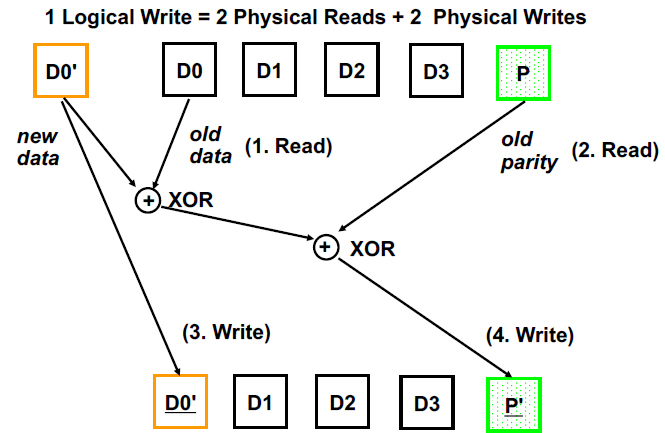
\includegraphics[width=0.309\textwidth]{CO6/Small Write Algorithm}
    \caption{Small Write Algorithm}
\end{figure}

\paragraph{RAID 5: High I/O Rate Interleaved Parity}
Inspiration for RAID 5: can't parallel write P. 

\begin{figure}[!htb]
    \centering
    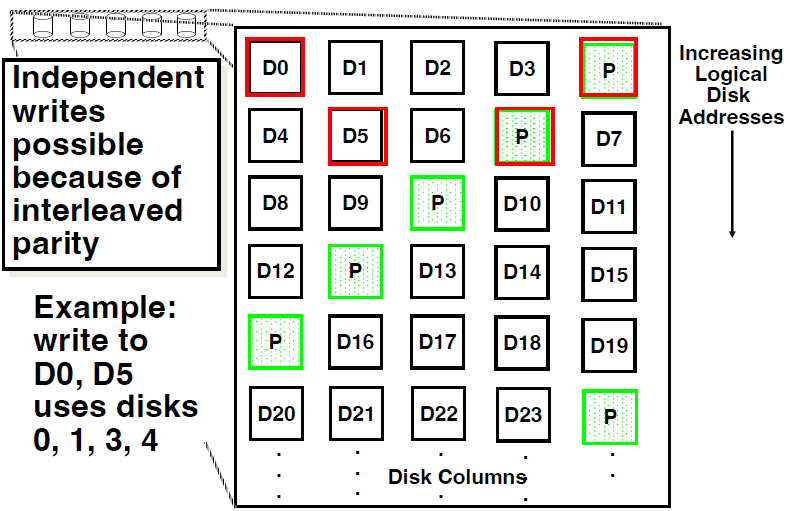
\includegraphics[width=0.309\textwidth]{CO6/RAID 5}
    \caption{RAID 5}
\end{figure}

\paragraph{RAID 6: P+Q Redundancy}
When a single failure correction is not sufficient, Parity can be generalized to have a second calculation over data and anther check disk of information.

\paragraph{Summary: RAID Techniques}

\begin{figure}[!htb]
    \centering
    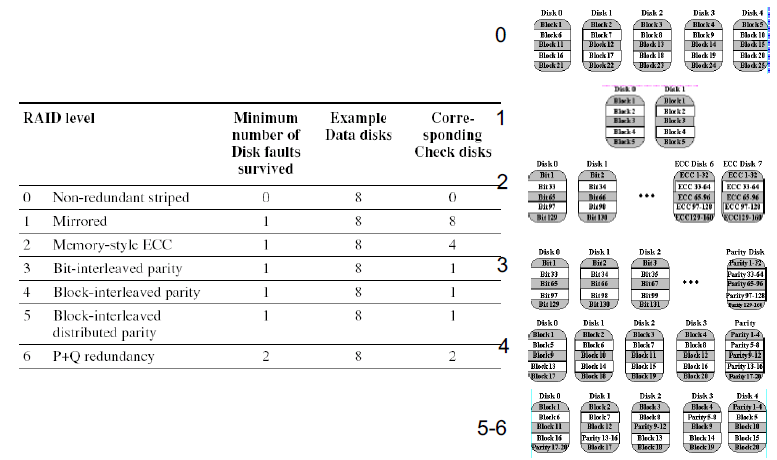
\includegraphics[width=0.42\textwidth]{CO6/RAID}
    \caption{RAID}
\end{figure}

\begin{itemize}
    \item Disk Mirroring, Shadowing (RAID 1)
    \item Parity Data Bandwidth Array (RAID 3)
    \item High I/O Rate Parity Array (RAID 5)
\end{itemize}

\subsection{Buses and Connections between Processors Memory and I/O Devices}
Buses and Other Connections
\subsubsection{Bus Basics}
\begin{figure}[!htb]
    \centering
    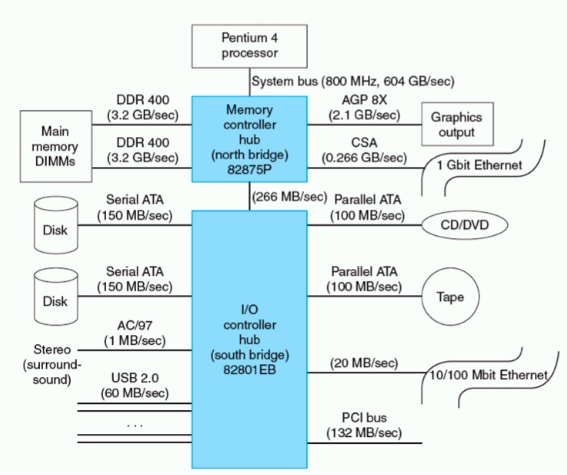
\includegraphics[width=0.309\textwidth]{CO6/Bus}
    \caption{Bus}
\end{figure}
Bus: Shared communication link (one or more wires)

A bus contains two types of lines:
\begin{enumerate}\small
    \item Control lines: signal requests and acknowledgments, and to indicate what types of information is on the data lines.
    \item Data lines: carry information (e.g., data, addresses, and complex commands) between the source and the destination.
\end{enumerate}

Bus transaction include two parts: sending the address and receiving or sending the data, which has two operations:
\begin{enumerate}\small
    \item input: inputting data from the device to memory
    \item output: outputting data to a device from memory
\end{enumerate}

\paragraph{Output Operation}\quad 
\begin{figure}[!htb]
    \centering
    \begin{subfigure}{0.42\textwidth}
        \centering
        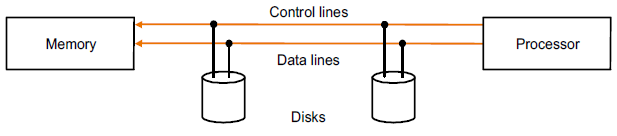
\includegraphics[width=\textwidth]{CO6/Output Operation1}
        \caption{\footnotesize  Initial a read for memory. Control lines signal a read request to memory, while the data lines contain the address. }
    \end{subfigure}
    \begin{subfigure}{0.42\textwidth}
        \centering
        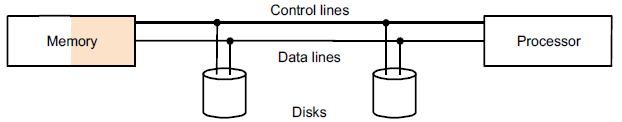
\includegraphics[width=\textwidth]{CO6/Output Operation2}
        \caption{\footnotesize  Memory access the data.}
    \end{subfigure}
    \begin{subfigure}{0.42\textwidth}
        \centering
        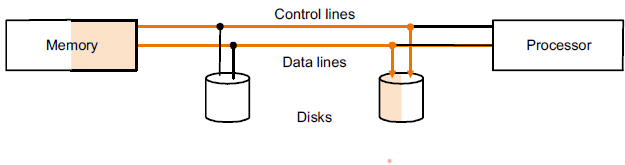
\includegraphics[width=\textwidth]{CO6/Output Operation3}
        \caption{\footnotesize  Memory transfers data and signal data is available. The device stores data as it appears on the bus.}
    \end{subfigure}
    \caption{Output Operation}
\end{figure}

\paragraph{Input Operation}\quad
\begin{figure}[!htb]
    \centering
    \begin{subfigure}{0.42\textwidth}
        \centering
        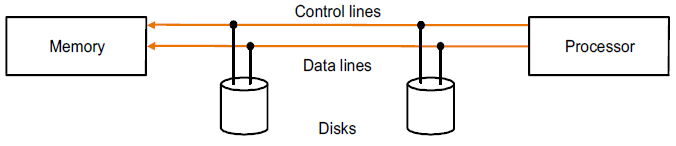
\includegraphics[width=\textwidth]{CO6/Input Operation1}
        \caption{\footnotesize Control lines indicate a write request for memory, while the data lines contain the address.}
    \end{subfigure}
    \begin{subfigure}{0.42\textwidth}
        \centering
        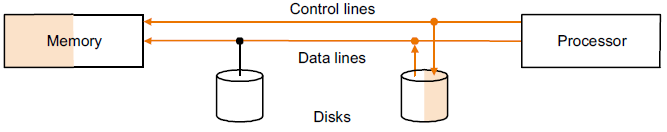
\includegraphics[width=\textwidth]{CO6/Input Operation2}
        \caption{\footnotesize When the memory is ready, it signals the device, which then transfers the data. The memory will store the data as it receives it . The device need not wait for the store to be completed.}
    \end{subfigure}
    \caption{Input Operation}
\end{figure}

\paragraph{Types of Buses}
\begin{itemize}\small
    \item Processor-memory : short high speed, custom design
    \item Backplane : high speed, often standardized
    \item I/O : lengthy, different devices, standardized
\end{itemize}

\subsubsection{Synchronous vs. Asynchronous}
\begin{itemize}\small
    \item Synchronous bus: use a clock and a fixed protocol, fast and small but every device must operate at same rate and clock skew requires the bus to be short
    \item Asynchronous bus: don't use a clock and instead use handshaking
    \item Handshaking protocol: A serial of steps used to coordinate asynchronous bus transfers.
\end{itemize}

\paragraph{Asynchronous example}
(握手协议)
\begin{figure}[!htb]
    \centering
    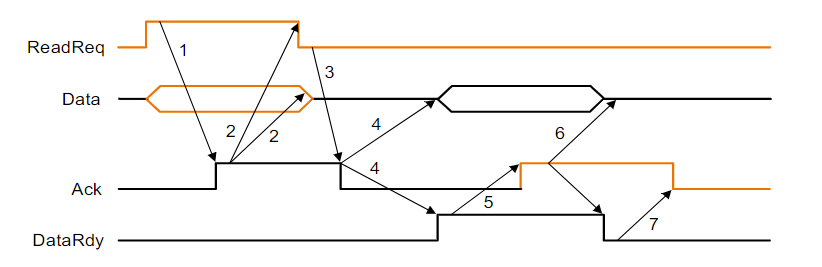
\includegraphics[width=0.42\textwidth]{CO6/Asynchronous example}
    \caption{Asynchronous example}
\end{figure}
\begin{enumerate}\small
    \item When memory sees the ReadReq line, it reads the address from the data bus, begin the memory read operation, then raises Ack to tell the device that the ReadReq signal has been seen.
    \item I/O device sees the Ack line high and releases the ReadReq data lines.
    \item Memory sees that ReadReq is low and drops the Ack line.
    \item When the memory has the data ready, it places the data on the data lines and raises DataRdy.
    \item The I/O device sees DataRdy, reads the data from the bus , and signals that it has the data by raising ACK.
    \item The memory sees Ack signals, drops DataRdy, and releases the data lines.
    \item Finally, the I/O device, seeing DataRdy go low, drops the ACK line, which indicates that the transmission is completed.
\end{enumerate}


\subsubsection{Bus Arbitration}
Obtaining Access to the Bus. Deciding which bus master gets to use the bus next. 

\begin{figure}[!htb]
    \centering
    \begin{subfigure}{0.42\textwidth}
        \centering
        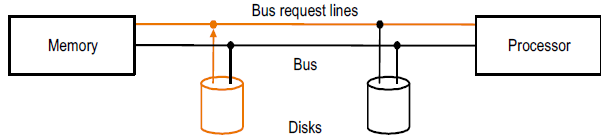
\includegraphics[width=\textwidth]{CO6/Bus Arbitration1}
        \caption{\footnotesize First, the device generates a bus request to inform the processor that it wants to use the bus.}
    \end{subfigure}
    \begin{subfigure}{0.42\textwidth}
        \centering
        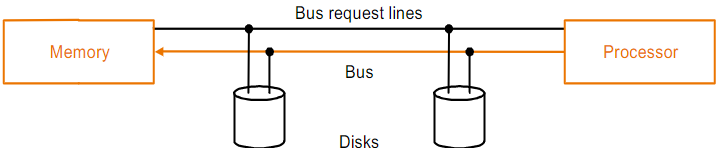
\includegraphics[width=\textwidth]{CO6/Bus Arbitration2}
        \caption{\footnotesize The processor responds and generates appropriate bus control signals. For example, if the devices wants to perform output from memory, the processor asserts the read request lines to memory.}
    \end{subfigure}
    \begin{subfigure}{0.42\textwidth}
        \centering
        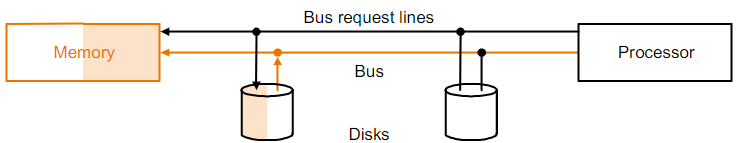
\includegraphics[width=\textwidth]{CO6/Bus Arbitration3}
        \caption{\footnotesize The processor also notifies the device that its bus request is being processed; as a result, the device knows it can use the bus and places the address for the request on the bus.}
    \end{subfigure}
    \caption{Bus Arbitration}
\end{figure}

In a bus arbitration scheme, a device wanting to use the bus signals a bus request and is later granted the bus. Four bus arbitration schemes:
\begin{enumerate}\small
    \item daisy chain arbitration (not very fair)
    \item centralized, parallel arbitration (requires an arbiter), e.g., PCI
    \item self selection, e.g., NuBus used in Macintosh
    \item collision detection, e.g., Ethernet
\end{enumerate}
Two factors in choosing which device to grant the bus:
\begin{enumerate}\small
    \item bus priority
    \item fairness
\end{enumerate}

% \subsubsection{Example}

% \paragraph{Synchronous vs Asynchronous Buses}\quad

% Assume: \begin{itemize}\small
%     \item The synchronous bus has a clock cycle time of 50 ns, and each bus transmission takes 1 clock cycle . 
%     \item The asynchronous bus requires 40 ns per handshake. 
%     \item The data portion of both buses is 32 bits wide.
% \end{itemize}

% Question: Find the bandwidth for each bus when reading one word from a 200-ns memory.

% Answer:
% \begin{enumerate}
%     \item synchronous bus: 
%     \item asynchronous bus:
% \end{enumerate}

% \paragraph{Increasing the Bus Bandwidth}
% Suppose we have a system with the following characteristic:
% \begin{enumerate}\small
%     \item A memory and bus system supporting block access of 4 to 16 32-bit words
%     \item A 64-bit synchronous bus clocked at 200 MHz, with each 64-bit transfer taking 1 clock cycle, and 1 clock cycle required to send an address to memory.
%     \item Two clock cycles needed between each bus operation.
%     \item A memory access time for the first four words of 200ns; each additional set of four words can be read in 20 ns. Assume that a bus transfer of the most recently read data and a read of the next four words can be overlapped.
% \end{enumerate}

% Question: Find the sustained bandwidth and the latency for a read of 256 words for transfers that use 4-word blocks and for transfers that use 16-word blocks. Also compute effective number of bus transactions per second for each case.

% Answer: 
% \begin{itemize}
%     \item the 4-word (1word 32bits) Block Transfers: each block takes
%     \begin{enumerate}\small
%         \item 1 clock cycle to send the address to memory
%         \item 200ns/(5ns/cycle) = 40 clock cycles to read memory
%         \item 2 clock cycles to send the data from the memory (64-bit synchronous bus)
%         \item Two clock cycles needed between each bus operation.
%     \end{enumerate}
%     This is a total of 45cycles.

%     There are $256/4 = 64$ blocks.

%     So the transfer of 256 words takes $45\times 64=2880$ clock cycles
    
%     \item the 16-word Block Transfers
% \end{itemize}



\subsection{Interfacing I/O Devices to the Memory, Processor, and Operating System}
Three characteristics of I/O systems: 
\begin{enumerate}\small
    \item \textbf{shared} by multiple programs using the processor.
    \item often use \textbf{interrupts} to communicate information about I/O operations.
    \item The low-level control of an I/O devices is \textbf{complex}
\end{enumerate}

Three types of communication are required:
\begin{enumerate}\small
    \item The OS must be able to give \textbf{commands} to the I/O devices.
    \item The device must be able to \textbf{notify} the OS, when I/O device
    \textbf{completed} an operation or has encountered an \textbf{error}.
    \item Data must be transferred between memory and an I/O device
\end{enumerate}

\subsubsection{Giving Commands to I/O Devices}
Two methods used to address the device:
\begin{itemize}\small 
    \item memory-mapped I/O: portions of the memory address space are assigned to I/O devices, and lw and sw instructions can be used to access the I/O port.
    \item special I/O instructions
\end{itemize}

\subsubsection{Communication with the Processor}
\begin{itemize}\small
    \item Polling: The processor periodically checks status bit to see if it is time for the next I/O operation.
    \item Interrupt: When an I/O device wants to notify processor that it has completed some operation or needs attentions, it causes processor to be interrupted.
    \item DMA (direct memory access): the device controller transfer data directly to or from memory without involving processor. 
\end{itemize}

\begin{figure}[!htb]
    \centering
    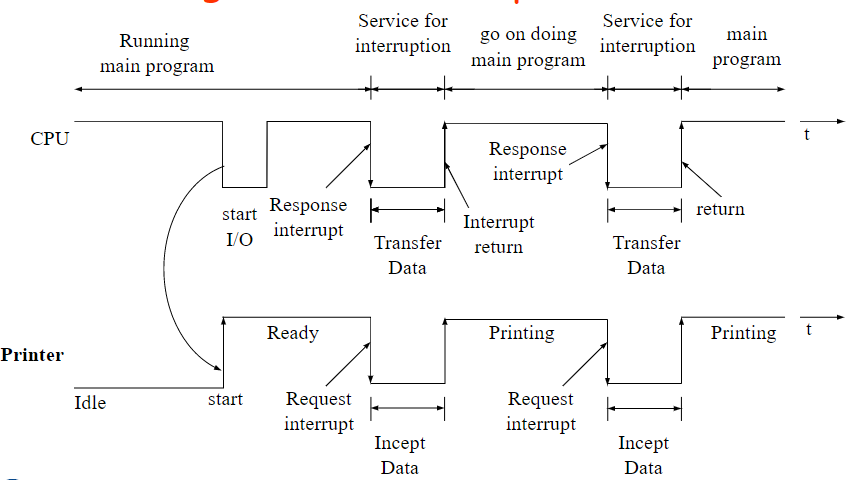
\includegraphics[width=0.42\textwidth]{CO6/Interrupt-Driven IO Mode}
    \caption{Interrupt-Driven I/O Mode}
\end{figure}

\paragraph{DMA Transfer Mode}\quad
A DMA transfer need three steps:
\begin{enumerate}\small 
    \item The processor sets up the DMA by supplying some information, including the identity of the device, the operation, the memory address that is the source or destination of the data to be transferred, and the number of bytes to transfer.
    \item The DMA starts the operation on the device and arbitrates for the bus. If the request requires more than one transfer on the bus, the DMA unit generates the next memory address and initiates the next transfer.
    \item Once the DMA transfer is complete, the controller interrupts the processor, which then examines whether errors occur. 
\end{enumerate}
\begin{figure}[!htb]
    \centering
    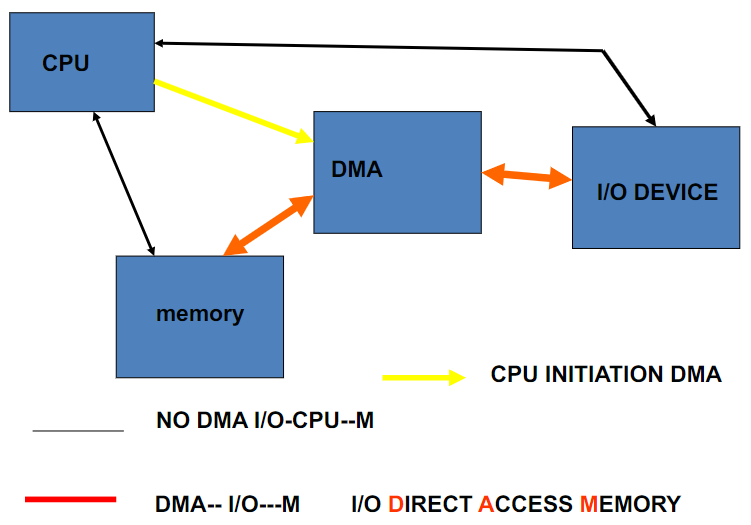
\includegraphics[width=0.42\textwidth]{CO6/DMA Transfer Mode}
    \caption{DMA Transfer Mode}
\end{figure}


\paragraph{Compare Polling, Interrupts, DMA}
The disadvantage of polling is that it wastes a lot of processor time. When the CPU polls the I/O devices periodically, the I/O devices maybe have no request or have not get ready. If the I/O operations is interrupt driven, the OS can work on other tasks while data is being read from or written to the device. Because DMA doesn't need the control of processor, it will not consume much of processor time.

% \subsubsection{Example}
% \paragraph{Overhead of Polling in an I/O System}

% \paragraph{Overhead of Interrupt-Driven I/O}

% \paragraph{Overhead of I/O Using DMA}


% \subsection{Designing an I/O system}


% \subsection{Real Stuff: A Typical Desktop I/O System}